% !TeX root = template-UNAMFC.tex

\subsection{Beamer}
	\subsubsection{Blocks y Multicols}


% -------------------------------------------------------------------------------------------
\begin{frame}[c]{Bloques de distintas índoles\footnotemark[1]}
				{Multicols para controlar tamaño  y otras cosas spongo}
%
\centering
	\begin{columns}
		\column{\squeezethree}
		\centering
			\begin{block}{block:  Es más limpio}
				Para multicols se  definieron mitades y tercias
				\begin{itemize} \itemsep.5em
					\item \backslash{squeezetwo}
					\item \backslash{squeezethree}
					\item \backslash{loosethree}
				\end{itemize}
			\end{block}
		\column{1.5\squeezethree}
		
			\begin{exampleblock}{exampleblock}
				El de colores más oscuros y letra azul
			    \begin{align*}
					\vb{E}^\text{exc}_k(\vb{r}) = & \vb{E}^\text{inc}(\vb{r}) + \sum_{\ell\neq k}^N \vb{E}^\text{ind}_\ell(\vb{r})\\
					\vb{E}^\text{ind}_\ell(\vb{r}) = & \int\dd^3 r' \mathbb{G}(\vb{r},\vb{r}') \times
					\int\dd^3 r''\mathbb{T}(\vb{r}'-\vb{r}_\ell,\vb{r}''-\vb{r}_\ell) \vb{E}_\ell^\text{exc}(\vb{r}'')\\
					\langle\vb{E}(\vb{r})\rangle = & \vb{E}^\text{inc}(\vb{r}) +  \sum_{\ell = 1}^N  \left(\prod_{k = 1}^N \int\dd^3 r_k \rho(\vb{R}) \vb{E}^\text{ind}_\ell(\vb{r})\right)
				\end{align*}
			\end{exampleblock}
	\end{columns}
\vskip1em
	\begin{columns}
		\column{.9\squeezetwo}
		\begin{alertblock}{alertblock}
			Colores claros y rojo para resaltar cosas
			\begin{align*}
				\langle \vb{E}_\ell^\text{exc}(\vb{r}'',\vb{R})\rangle_\ell =& \vb{E}^\text{inc}(\vb{r}'')
				+ \sum_{\substack{m =1 \\ m\neq \ell}}^N  \int\dd^3 r' \mathbb{G}(\vb{r}',\vb{r}'') \times \notag\\
				& \int\dd^3 r'''\int \dd^3 r_m \rho(\vb{r}_m) \mathbb{T}(\vb{r}'-\vb{r}_m,\vb{r}'''-\vb{r}_m) \langle \vb{E}_m^\text{exc}(\vb{r}'',\vb{R})\rangle_{\ell,m}
				\\
				\langle \vb{E}_m^\text{exc}(\vb{r}'',\vb{R})\rangle_{\ell,m},
				&= \prod_{\substack{n =1 \\ n\neq \ell,m}}^N  \int\dd^3 r_n \rho(\vb{R}|\vb{r}_\ell,\vb{r}_m) \vb{E}^\text{exc}_n(\vb{r}'')
			\end{align*}
		\end{alertblock}
		\column{.9\squeezetwo}
	\end{columns}	% 

%


    \begin{textblock*}{75mm}(180mm,80mm)
    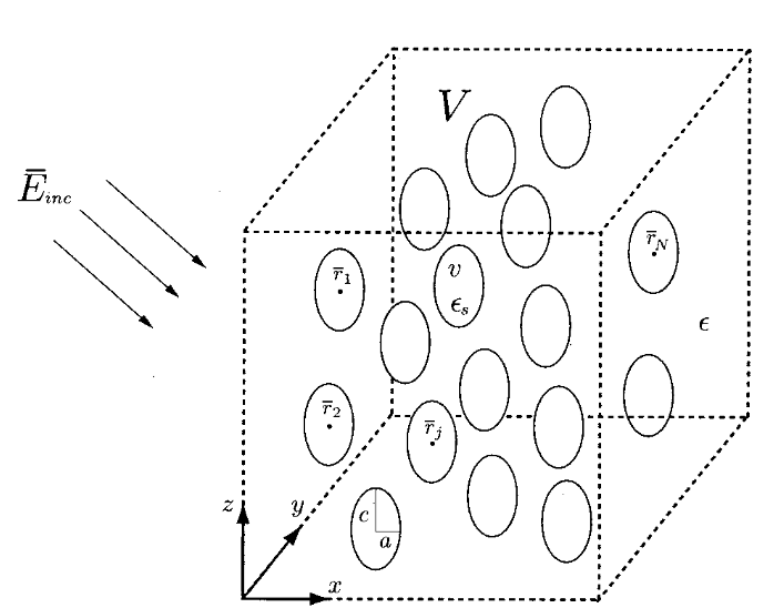
\includegraphics[width=75mm]{img/1-multiple.png}
\end{textblock*}
\begin{textblock*}{22mm}(175mm,120mm)
    \begin{flushright}
    \scriptsize
    \fullcite{ao_analytical_2002}
    \end{flushright}
\end{textblock*}


    \begin{textblock*}{80mm}(145mm,137.5mm)
        \begin{flushleft}
        \scriptsize
        \rule{30mm}{.5pt}\\
        \footnotemark[1]\fullcite{garcia2012multiple}
        Esto es un textlock aislado
    \end{flushleft}
     \end{textblock*}

\end{frame}